\RequirePackage{etex}
\RequirePackage{fix-cm} % For custom font shaping

% Document class
\documentclass[pdftex, 11pt, a4paper, oneside, english]{memoir}

% Page styling
\let\footruleskip\undefined
\usepackage{fancyhdr}
\pagestyle{fancy}

% English language package
\usepackage[english]{babel}

% UTF-8 characters
\usepackage[utf8]{inputenc}

% Package for dummy text
\usepackage{lipsum}

% Colors for chapters and table of content
\usepackage[table,xcdraw]{xcolor}
\definecolor{ThemeColor}{RGB}{0, 154, 242} % Blue
\definecolor{BlackColor}{RGB}{0, 0, 0} % Black

% Table packages
% Merge cells i tables
\usepackage{multirow}
\usepackage{makecell}
\usepackage{tabularx}

% PDF propeties (fx. hyperlinks, pdftitle)
\usepackage[hyphens]{url}
\usepackage[bookmarks=true,bookmarksnumbered=true,citecolor=black,colorlinks=true,hyperfigures=true,hyperfootnotes=true,hyperindex=true,linkcolor=black,urlcolor=blue]{hyperref}

% BibTeX = bibliography
% ALWAYS USE \citep{} or something like:
% \citep[see this baws article]{fooArticle}
\usepackage[semicolon,authoryear,round]{natbib}
\bibliographystyle{plainnat}

% Package for editing captions. Fx for figures and code listings
\usepackage[textfont={footnotesize,sl}]{caption}

%Package for MATLAB code
\usepackage[framed, numbered]{mcode}

% Package for more elegant math
\usepackage{amsmath}
\usepackage{xfrac} % for \sfrac command

% Styles
% Package for setup of chapters and sections
\usepackage{titlesec}


% % % % % % % % % % % % % % CHAPTER  % % % % % % % % % % % % % % % % % % % % % %
% Define fontsize for the numbering of the chapters
\newcommand{\ChapterNumbering}{
    \usefont{\encodingdefault}{\rmdefault}{b}{n}
    \fontsize{35}{45}\normalfont\color{ThemeColor}}

% Chapter numbers in margin
\chapterstyle{hangnum}

% Modifying "\chapterstyle{hangnum}"
% Changing vertical position of chapter headline
\renewcommand*{\chapterheadstart}{\vspace*{-20pt}}

% Color setup for chapters
% Title color
\renewcommand*{\chaptitlefont}{\bfseries\Huge\color{BlackColor}}
% Number color
\renewcommand{\chapnumfont}{\normalfont\ChapterNumbering\color{ThemeColor}}




% % % % % % % % % % % % % % SECTION  % % % % % % % % % % % % % % % % % % % % % %
% Section numbers in margin
\hangsecnum

% Color setup for sections
% Title color
%\renewcommand\thesection{\color{ThemeColor}\thechapter.\arabic{section}}
\renewcommand\thesection{\thechapter.\arabic{section}}

% Set numbering depth of sections
\setsecnumdepth{subsubsection}

% Set the depth of sections included in table of contents
\settocdepth{subsection}



% Clear all header an footer fields
\fancyhf{}


% % % % % % % % % % % % % % HEADER % % % % % % % % % % % % % % % % % % % % % % %
% Delete headruler
\renewcommand{\headrulewidth}{0pt}

% Insert picture in left side on even pages and right side on odd pages
\fancyhead[R]{
\includegraphics[height=40pt]{figure/header/header}}



% % % % % % % % % % % % % % FOOTER % % % % % % % % % % % % % % % % % % % % % % %
% Insert pagenumber on right side of even page, left side of odd page
\fancyfoot[R]{\thepage}

\setlength\headheight{44.1pt}

%\setcounter{page}{1}

%%%%%%%%%%%%%%%%%%%%%%%%%%%%%%%%%%%%%%%%%%%%%%%%%%%%%%%%%%%%%%%%%%%%%%%%%%%%%%%%
%                       Custom for figures (myFigure etc.)                     %
%                     			      	        		                       %
%%%%%%%%%%%%%%%%%%%%%%%%%%%%%%%%%%%%%%%%%%%%%%%%%%%%%%%%%%%%%%%%%%%%%%%%%%%%%%%%

% Include image and graphic
\usepackage{graphicx}

% Package for wrapping figures in text
\usepackage{wrapfig}

% Set the path where LaTeX looks for pictures.
\graphicspath{{figure/}}

% You need a newsubfloat element to use subcaption
\newsubfloat{figure}

% Command to set caption styles
\captionsetup[figure]{
    labelfont=bf
}

\captionsetup[table]{
    labelfont=bf
}

% from the old preamble
\captionnamefont{\bfseries\small}
\captiontitlefont{\itshape\small}
\subcaptionlabelfont{\bfseries\small}
\subcaptionfont{\itshape\small}


% Command \myFigure{filename}{caption}{label}{width} 
% for inserting a new figure.
\newcommand{\myFigure}[4]
{ 
    \begin{figure}[ht] 
        \centering 
        \includegraphics[width=#4\textwidth]{#1} 
        \caption{#2} 
        \label{#3} 
    \end{figure}
} 
 
% Insert a figure wraped in text (left/right)
% Command \myWrapFigure{filename}{caption}{label}{width}{r/l}
\newcommand{\myWrapFigure}[5]
{ 
    \begin{wrapfigure}{#5}{#4 \textwidth}
        \begin{center}
            \includegraphics[width=#4\textwidth]{#1}
        \end{center}
        \caption{#2}
        \label{#3} 
    \end{wrapfigure}
}
 
% Insert two figures side by side, with a caption covering both and a subcaption for each figure. OBS: scaled for 50 % text width both
% Command \mySubFigure{filename1}{filename2}{caption}
% {subcaption1}{subcaption2}{label}{sublabel1}{sublabel2}
\newcommand{\mySubFigure}[9]
{
    \begin{figure}[ht]
        \centering
        \subbottom[{#4}\label{#7}]%
            {\includegraphics[width=0.5\textwidth]{#1}}\hfill
        \subbottom[{#5}\label{#8}]%
            {\includegraphics[width=0.5\textwidth]{#2}}
        \caption{#3}
        \label{#6}
    \end{figure}
}


% Keeps floats in the section. 
% Help control place to put pix
\usepackage[section]{placeins}


%Package with enumirate command with extra options (used within cells of tabular)
\usepackage[inline]{enumitem}
\usepackage[]{todonotes}


% new commands for individually colored todo 
\newcommand{\todowex}[2]{
\todo[#1, color=blue!40]{#2 \\- Wex}
}
\newcommand{\todojens}[2]{
\todo[#1, color=green!40]{#2 \\- Jens}
}
%\input{style/code}
%%%%%%%%%%%%%%%%%%%%%%%%%%%%%%%%%%%%%%%%%%%%%%%%%%%%%%%%%%%%%%%%%%%%%%%%%%%%%%%%
%                           Custom Commands                                    %
%                                                                              %
%%%%%%%%%%%%%%%%%%%%%%%%%%%%%%%%%%%%%%%%%%%%%%%%%%%%%%%%%%%%%%%%%%%%%%%%%%%%%%%%

%%%%% FIGURES %%%%%
% The following commands are defined in: style/figure

% Insert a new figure:
% \myFigure{filename}{caption}{label}{width}
% width is ratio of textwidth, so it should be between 0.1 and 1

% Insert a figure wraped in text (left/right)
% \myWrapFigure{filename}{caption}{label}{width}{l/r}
% width is ratio of textwidth, so it should be between 0.1 and 1
% l/r: l = left, r = right

% Insert two figures side by side, with a caption covering both and a subcaption for each figure. OBS: scaled for 50 % text width both
% Command \mySubFigure{filename1}{filename2}{caption}
% {subcaption1}{subcaption2}{label}{sublabel1}{sublabel2}



%%%%% TABLES %%%%%
% Command \myTable{caption text}{refrence label}{input filename: eq <tables/myTable>}
% for inserting tables


%%%%% CODE LISTING %%%%%
%\begin{lstlisting}[language=Matlab, caption={Dette er et eksempel på hvordan du skal bruge listing}, label=list_me_like_a_baws]
%
%	INSERT CODE HERE
%
%\end{lstlisting}

% For more info go to http://ctan.org/pkg/listing



%%%%% EQUATIONS / MATH %%%%%
% For info in the user guide at http://ctan.org/pkg/amsmath
% Feel free to add ninja tricks to this guide



%%%%% BibTeX %%%%%
% To cite some article use:
% \citep{fooArticle} or
% \citep[see this baws article]{fooArticle}

% OBS: remember to add article to "bibliografi.bib" using syntex of the examples in the file.



%%%%% Nomenclature %%%%%
% When introducing a new symbol add it to the nomenclature by:
% \nomenclature{symbol}{description}
% remember to put symbol in mathmode if necessary
% OBS: if you need to add more the one symbol you have to add a "%" at the end of every \nomenclature use except for the last one. See example below:
%
%	\begin{equation}
%		e=m \cdot c^2
%	\end{equation}%
%	\nomenclature{$e$}{Energy}%
%	\nomenclature{$m$}{The mass}%
%	\nomenclature{$c$}{The speed of light. 299 792 458 $\frac{m}{s}$}

%%%%% COLOR %%%%%
\definecolor{deadlinecolor}{HTML}{FD6864}
\definecolor{reviewcolor}{HTML}{9698ED}

%%%%% TEXT COMMANDS %%%%%
\newcommand{\prbl}{Problematic} % For the lulz

%%%%% MATH COMMANDS %%%%%
\newcommand{\degree}{^\circ}

% Command \myTable{caption text}{refrence label}{input filename: eq <tables/myTable>}
% for inserting tables
\newcommand{\myTable}[3]
{ 
    \begin{table}[h]
    \centering
    \caption{#1}
    \label{#2}
        \input{#3}
    \end{table}
}
% Example on content in table file
%
%    \begin{tabular}{rll}
%    \multicolumn{1}{c}{\textbf{Tapsstørrelse}} &
%    \multicolumn{1}{c}{\textbf{Målt beregningstid}} \\ \hline
%       1      &  35,6  $\mu s$     \\[0.05cm] 
%       2      &  36,5  $\mu s$     \\[0.05cm] 
%       5      &  32,0  $\mu s$     \\[0.05cm] 
%       8      &  32,0  $\mu s$     \\[0.05cm] 
%       10     &  32,0  $\mu s$     \\[0.05cm] 
%       20     &  32,5  $\mu s$     \\[0.05cm] 
%       50     &  69,0  $\mu s$     \\[0.05cm] 
%       80     &  101,5 $\mu s$     \\[0.05cm] 
%       100    &  124,5 $\mu s$     \\[0.05cm] 
%       200    &  240,5 $\mu s$     \\[0.05cm] 
%       500    &  587   $\mu s$     \\[0.05cm] 
%       800    &  932   $\mu s$     \\[0.05cm] 
%       1000   &  1164  $\mu s$     \\[0.05cm] 
%       1024   &  1192  $\mu s$     \\[0.05cm]
%       \hline
%       512    &  601   $\mu s$     \\[0.05cm]
%       513    &  605   $\mu s$     \\
%    \end{tabular}



% Geometry for frontpage
\usepackage{geometry}

% For traceability matrix
\usepackage{longtable}
\usepackage{rotating}

\begin{document}

	\begin{titlingpage}
		% Frontpage goes here
		\newgeometry{left=3cm,bottom=0.1cm}

\centerline{\Huge\bfseries\color{ThemeColor} Graphikos}

\vspace{1em}
\centerline{\Large\bfseries\color{BlackColor} Course work PLPA 2016 Q4}



\vspace{5em}
\centerline{\large\bfseries\color{BlackColor}}
\centerline{\large\color{BlackColor}Department of Engineering - Aarhus University}

\vspace{0.5em}
\centerline{\large\color{BlackColor} May 25, 2016}

\vspace{25em}

\begin{center}
   \begin{tabular}{ l p{3cm} l l }
   Stud. no.: 201270782 && Torben Werenberg Vogt & \\\hline
   & & \\
   Stud. no.: 201270097 && Simon Østergaard Kristensen & \\\hline
   & & \\
   Stud. no.: 201270762 && René Rotvig Jensen & \\\hline
   & & \\
   Stud. no.: 201270860 && Kristoffer Sloth Gade & \\\hline
   \end{tabular}
\end{center}
\thispagestyle{empty} % No header and footer on this page
\restoregeometry


	\end{titlingpage}
	


    % Table of contents
    \tableofcontents*	% The star keeps TOC from indexing itself

    \chapter{Introduction}
\label{chp:intro}

This report and the developed image compression and transmission project solves the assignment given in the \emph{mini-project 6} in the course \emph{Wireless Sensor Network and Electronics}.

The project concerns with transferring an image between two TelosB motes. The image will be transferred both with and without compression. Three different lossy compression algorithms has been developed and implemented on the TelosB motes. 

This report will explain the theory of the project. Furthermore it will analyze energy consumption, present the results and discuss the advantages and disadvantages of using compression.
    \chapter{Theory}
\label{chp:theory}

In this chapter the theory of the project will be described. This includes the compression, energy consumption and radio communication.

\section{Compression}
In general image compression is about the removal of data in order to minimize a file size. This can be done lossless or lossy, depending on the use and importance of the data.

\subsection{Lossy and lossless compression}
When using a lossless image compression, every bit information in the file remains when compressed, and it will be just like the original when decompressed. This technique is preferred when compressing spreadsheet or text files, as it can be useless, if some of the text i missing. It is also a more complex compression method so if high quality is not a factor, then a lossy compression is maybe preferred 

In the lossy compression, some data is permanently removed which reduces the size of the image file. This means that when the image is decompressed only a part of the original image is still there. It is not sure that the user will not notice the missing information, but it will cause a lower quality in the picture. This compression is widely used in video and sound where the quality can be reduced.  

\subsection{N-bit compression}
In this project three n-bit compressions has been used namely 1-bit, 2-bit and 4-bit compression. in figure \ref{fig:NbitCompression} an example of a 1-bit compression is shown. When it is compressed the least significant bit (LSB) is removed in every byte. This resulting in less data in the image. When it is decompressed, there is added a \emph{0} is added on the least significant bit in every byte, so the image get the same length. 

\myFigure{NbitCompression}{1-bit compression.}{fig:NbitCompression}{0.7}

The image with the compression will loose some details and will generally be in a lower quality than the original image during the lack of information the compression has cost. So if the quality of a picture needs to be hight, this is not the best compression to do.  

\section{Energy consumption}
When looking at wireless sensor networks, energy consumption is an important issue. When transferring data there is a consumption of energy, this can be affected by the size of the data being transferred. When transferring data between two TelosBs, the level of energy consumptions needs to be at your attention because the TelosB has a limited amount of battery capacity. The challenge is to know when and how to use the radio communication.

\section{New Energy consumption}
When talking about sensor nodes the energy supply is a crucial factor. Batteries that runs the sensor nodes has small capacity and recharging them can be difficult and complicated. Hence the energy consumption must be controlled in the best way, to keep a low energy consumption.
The main consumers of energy are:
\begin{itemize}
	\item[--] The controller
	\item[--] Radio front ends
	\item[--] To some degree the memory
	\item[--] The sensors, depending on the type
\end{itemize}
	 
To reduce the energy consumptions a low-power chip is preferred, but it is only one half of the picture. If the chip is used improperly it will consume as much energy as an non low-power chip.

Avoiding this can be accomplished by observation of the wireless sensor node, and make sure that it has nothing to do most of the time. This can be handled by use of the controller's different states. The typical states of a controller is:
\begin{itemize}
	\item[--] \textbf{\emph{active}:} Working 
	\item[--] \textbf{\emph{idle}}: Ready to communicate 
	\item[--] \textbf{\emph{sleep}}: Waiting.
\end{itemize}

Using states is a core technique to reduce the energy consumption in wireless sensor nodes. Some sensors also uses \emph{deeper sleep} to save even more energy. When working with deeper sleep, it has to be taken into account that it takes more time and energy to make the controller wake up and be fully operational again.

Another way of controlling the energy consumption intead of states, is to scale the voltage as required. This can be done by using the full power of the microcontroller and get the task done as fast as possible, and go back to low energy consumption again. By doing this the task is done as fast as possible, and the high energy consumption is active in a limited time only. This may not be the most energy effecient approach, as the task may be computed at a low energy level. By using Dynamic Voltage Scaling(DVS) a task will be computed only at the speed needed of the task, to get it done before a given deadline.

\subsection{Memory}
 The most relevant kinds of memory when looking from an energy perspective is the FLASH memory and in generally on-chip memory. The off-chip RAM is not interesting, because they are rarely used, and is usually powered of the energy that runs the controller.
 The FLASH memory can have heavily influence on the lifetime of a controller. Writing and reading to the FLASH memory is tasks that consume energy, specially writing to it consumes a lot. The reason why is that is a more complicated process that the read process and it is furthermore time consuming.
 If it can be avoided it would be the best solution.  
 
 \subsection{Radio transceivers}
  
  There is two tasks for a a radio transceiver: transmitting and receiving data between nodes. Just like controllers radio transceiver works in different modes. The most common is \emph{turned on} or \emph{turned off}. To ensure a low energy consumption the transceivers has to be turned off most of the time, and only turned on when it is required. this meaning that they work at a low duty cycle.
  This increase the level of complexity, power overhead and time. 
  
  \subsubsection{Energy consumption during transmission}
  When transmitting the energy consumed is due to two sources. the first soruce is the RF signal that is generated which mostly depends on target distance, the chosen modulation and the transmission power which is one of the most crucially decisions when transmitting a packet.. The second source is due to electronic components. These costs are mostly constant.
  
  \subsection{Sensors and actuators}
  It is difficult to state guidelines for the energy consumptions for sensors and actuators due to the wide diversity of these devices.
  
 
\section{Radio communication}
    \chapter{Implementation} 
\label{chp:impl}

This chapter explains the design and implementation of the application and the choices made during the development.

\section{Multi paradigm}
The application uses the functional programming language Scheme together with the imperative language C\#. This is done by using \emph{IronScheme} which is an implementation of Scheme that targets .NET. This allows to call Scheme functions directly from C\# and hence combine the two languages.

\section{User interface in C\# WPF}
C\# WPF was used for developing the graphical user interface which made it possible to create the required interface that allowed the user to draw different objects.

This was done using Model-View-ViewModel(MVVM) architecture to separate the graphical user interface from the business logic. This was implemented using the MVVM framework CaliburnMicro. Using MVVM ensured that the business logic was loosely coupled with the view through data-binding and therefore easier to test. This is illustrated in figure \ref{fig:mvvm}

\myFigure{mvvm.png}{Model-View-ViewModel}{fig:mvvm}{1} 

The class diagram shown in figure \ref{fig:class} illustrates the essential design and classes used. The ShellView presents the content for the user and is updated through data-binding by the ShellViewModel. ShellViewModel depends on the two interfaces IShemeHandler and IBitmapDrawing. By only depending on interfaces, testability is ensured as mocks can be used instead of concrete implementations. 

SchemeHandler handles the evaluation of the scheme code by using IronScheme. BitmapDrawing is used for drawing single pixels and text on the bitmap.

\myFigure{class.png}{UML class diagram}{fig:class}{0.6} 

Furthermore the C\# WPF also holds the state of the bounding-box in the ShellViewModel. This was chosen to keep the scheme code stateless. If a bounding-box was set by the user in the input field then the view model added a filter call to the called scheme function. By doing this the scheme code filtered away all the coordinates outside the bounding-box.

\section{Drawing Engine in Scheme}
Scheme was used for developing the drawing engine. This allowed for fast and stateless computation of the graphics being shown in the user interface. 

For drawing lines in the application the Bresenham’s line algorithm was used. This algorithm can draw a line between two points. The circle Midpoint algorithm was used for drawing circles. The implementation of the circle function is shown in listing \ref{lst:circle}. The function takes three parameters, the center coordinates and the radius. First x, y and d is created. \emph{x} is defined as 0, and are used as a counter \emph{y} is a copy of r, and is used in the algorithm calculations. Final \emph{d} is  a decision parameter and decides the calucation of paramters of the recursive call. The stop condition is when \emph{x} is bigger than \emph{y}, then the the last element \emph{'()} is returned at the list composed and returned.

The circle function is implemented with classic recursion. Tail recursion could also have been used but in this case classic recursion was sufficient. If the circles instead had to be drawn on a bigger bitmap the classic recursive calls could lead to stack overflow.


\begin{lstlisting}[caption={Scheme function circle}, label=lst:circle]
(define (circle centerX centerY r)
(let((x 0) (y r) (d (/ (- 5 (* r 4)) 4)))
(letrec ((GetCircleCoor (lambda (x y r d)
(if (<= x y)
(if (< d 0)    
(cons (+ centerX x) (cons (+ centerY y)                                                
(cons (- centerX x) (cons (+ centerY y)
(cons (+ centerX x) (cons (- centerY y)         
(cons (- centerX x) (cons (- centerY y)
(cons (+ centerX y) (cons (+ centerY x)
(cons (- centerX y) (cons (+ centerY x)
(cons (+ centerX y) (cons (- centerY x)
(cons (- centerX y) (cons (- centerY x)  
(GetCircleCoor (+ x 1) y r (+ d (+ (* x 2) 1)))))))))))))))))))
(cons (+ centerX x) (cons (+ centerY y)                                                
(cons (- centerX x) (cons (+ centerY y)
(cons (+ centerX x) (cons (- centerY y)         
(cons (- centerX x) (cons (- centerY y)
(cons (+ centerX y) (cons (+ centerY x)
(cons (- centerX y) (cons (+ centerY x)
(cons (+ centerX y) (cons (- centerY x)
(cons (- centerX y) (cons (- centerY x)  
(GetCircleCoor (+ x 1) (- y 1) r (+ d (+ (* 2 (- x y)) 1))))))))))))))))))))
'() ))))
(GetCircleCoor x y r d))))   
\end{lstlisting}

A function where tail recursion was required is the implemented function \emph{fill}. Which is a function that can fill an object with a color in the application. The difference between classic and tail recursion is
\begin{itemize}
	\item[--] \textbf{Classic recursion} makes the recursive calls before the actual processing
	\item[--] \textbf{Tail recursion} does the processing before the recursive call.  
\end{itemize}

fill was first created with classic recursion but this gave a stack overflow as two many function calls were made. Instead tail recursion was used so that the compiler could optimize this function and avoid stack overflow.  This is because the scheme compiler is able to very effectively optimize tail recursion compared to classic recursion.

\begin{lstlisting}[caption={Scheme function fill}, label=lst:fill]
(define (fill c g)
(letrec ((fillCoor (lambda(g x)
(if (or (or (null? g) (null? (cdr g)) (null? (cddr g))) (null? (cdddr g)))
(append x (cons c '()))
(fillCoor (cddddr g)
(append (line (car g)
(cadr g)
(car (cddr g))
(car (cdddr g))) x))
))))
(fillCoor g '())))
\end{lstlisting}

Furthermore the \emph{fill} function uses high order programming as functions are passed as parameters. 

The function is shown in listing \ref{lst:fill} and takes the parameters \emph{c} and \emph{g} where \emph{c} is the color and \emph{g} is a function that draws an object. It runs through the list that the function returns and uses the line algorithm to draw lines between two opposite coordinates. This implementation was chosen as it was simple approach to create a fill function even though some redundant coordinates might be included. 

Another function that uses high order programming is the draw function. The function was designed as a variadic function that takes a variable amount of other functions and combines them. The function can be called with a color but this is optional. The part where you can see the varidic parameter is shown 
in listing \ref{lst:draw}
 
\begin{lstlisting}[caption={Part of scheme function draw }, label=lst:draw]
(define (draw . g)
...
\end{lstlisting}
    \chapter{Test}
\label{chp:test}

Testing is an important part of a project. It is used to check the behavior of the source code, and to make sure the functionality is correct. The initially creation time is high. In the end it saves time and cost in the development process because errors are easier and earlier discovered.

\section{Test Strategy}
In this project testing is divided into two parts. One part is the test of the drawing engine in Scheme. The other part is test of the WPF application in C\#.

\section{Scheme test}
The test of the drawing engine in scheme  is implemented i the Scheme.ss file. For each function, \emph{line, rectangle, circle, fill, bounding-box text-at} and \emph{draw} a test is made. To test a function in scheme, the output of a function is compared to the expected value of the output. To do this, \emph{equal?} is used. This is shown i listing \ref{equal}.

\begin{lstlisting}[caption={Comparison of actual output with the expected output with equal?}, label=equal]
(and (equal? (candidate 0 0 8 8) '(0 0 1 1 2 2 3 3 4 4 5 5 6 6 7 7 8 8)))
\end{lstlisting}

This example is taken from the \emph{test-line} function. The line function takes 4 parameters, \emph{x, y, x2} and \emph{y2}. The test feeds the parameter 0, 0, 8 and 8, and compares to see if it is equal to what is expected. The expected value is in this example '0 0 1 1 2 2 3 3 4 4 5 5 6 6 7 7 8 8'. When the test function is written af TestRun function to run the test is made. Listing \ref{testrun} shows the run af a function along with it's test function. 

\begin{lstlisting}[caption={TestRunLine}, label=testrun]
(define TestRunLine (test-line line))
\end{lstlisting}

\emph{test-line} is the test function and \emph{line} is the function that needs to be tested. When \emph{TestRunLine} is executed it will return a \#t for true or a \#f for false.

\section{C\# Unit Testing}
The C\# WPF application has been tested by using xUnit.net and resharper xunit test runner. The tests are structured by "Arrange", "Act" and "Assert". The tests are placed in a separate test project called GraphikosTests. Every method is tested for all the successful scenarios and all the unsuccessful scenarios.

In some tests a mock is needed which the framework Moq is used to do. The mocks are used to separate the different classes. The mocks are effective to separate the individual classes which results in unit tests and not integration tests.

The maintenance of the code is made lesser error prone with the unit tests. This could result in a faster development time.

To be able to test the bitmaps which are generated or changed by different classes. The bitmaps are converted to a byte array and compared with another byte array which they should match. If they don’t match the bitmaps the functions are generating is wrong. This testing method was chosen because bitmaps don’t have any relevant properties to test on.
    \chapter{Results}
\label{chp:results}

In this chapter the results of the project will be presented. This includes measurements of four transmissions of the image. No compression, 1-bit compression, 2-bit compression and 4-bit compression.

To acquire the results, an image was transferred between the two TelosB motes, one as a sender and another as a receiver. These was implemented as described in chapter \ref{chp:impl}

Three different compressions was developed, and each with a different result, as expected. As shown i figure \ref{fig:one}, \ref{fig:two} and \ref{fig:four}.

\todo{indsæt rette billeder}
\begin{figure}[h]
	\centering
	\begin{subfigure}{0.3\textwidth}
		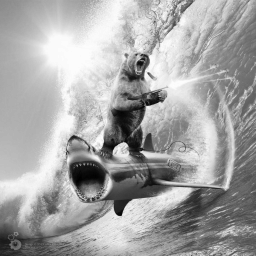
\includegraphics[width=\textwidth]{oneBit}
		\caption{1-bit compression}
		\label{fig:one}
	\end{subfigure}
	\begin{subfigure}{0.3\textwidth}
		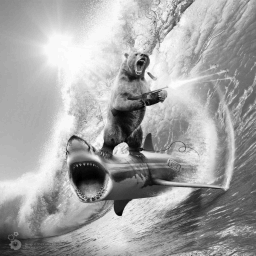
\includegraphics[width=\textwidth]{twoBit}
		\caption{2-bit compression}
		\label{fig:two}
	\end{subfigure}
	\begin{subfigure}{0.3\textwidth}
		\includegraphics[width=\textwidth]{fourbit}
		\caption{4-bit compression}
		\label{fig:four}
	\end{subfigure}
	\caption{Pictures of animals}\label{fig:animals}
\end{figure}


To measure the voltage over the mote and the transmission time, an oscilloscope was used. Figure \ref{fig:receiverresult} shows the measurement of the time for transferring with no compression. 

\myFigure{senderResultconverted}{Measured time for no compression for \emph{Receiver Mote}}{fig:receiverresult}{0.5}


The table below shows all measurements and calculations of the three compressions and the one without compression. The battery voltage for the sender was measured to $3.028V$ and the resistor to $9.93\Omega$. For the receiver the battery voltage was $3.214V$ and the resistor was measured to of $9.98\Omega$.

\vspace{0.5cm}
{\renewcommand{\arraystretch}{1.2}
\noindent
\begin{tabular}{l l l l r r r r}
	Sender           	& $V_{avg}$ & $t$ & $V_{mote}$  & $I_{mote}$ & $W_{mote}$ & Energy cons. & Eenergy saved \\
	& $\lbrack mV\rbrack$ & $\lbrack sec\rbrack$ & $\lbrack V\rbrack$  & $\lbrack V \rbrack$ & $\lbrack W\rbrack$ & $\lbrack J \rbrack$ & $\lbrack \% \rbrack$ \\ \hline
	No compr.	 & 0.194 & 25.2 & 2.834 & 0.020 & 0.055 & 1.395 & -\\
	1-bit compr. & 0.192 & 24.5 & 2.836 & 0.019 & 0.055 & 1.343 & 3.728\%\\
	2-bit compr. & 0.193 & 23   & 2.835 & 0.019 & 0.055 & 1.267 & 9.176\%\\
	4-bit compr. & 0.194 & 18.2 & 2.834 & 0.020 & 0.055 & 1.008 & 27.742\%\\
	
	&&&&&&& \\

	Receiver           	& $V_{avg}$ & $t$ & $V_{mote}$  & $I_{mote}$ & $W_{mote}$ & Energy cons. & Eenergy saved \\
	& $\lbrack mV\rbrack$ & $\lbrack sec\rbrack$ & $\lbrack V\rbrack$  & $\lbrack V \rbrack$ & $\lbrack W\rbrack$ & $\lbrack J \rbrack$ & $\lbrack \% \rbrack$ \\ \hline
	No compr.	& 0.201 & 25.2 & 3.013 & 0.020 & 0.060 & 1.529 & -\\
	1-bit compr. & 0.201 & 24.5 & 3.013 & 0.020 & 0.060 & 1.487 & 2.747\%\\
	2-bit compr. & 0.2   & 23   & 3.014 & 0.020 & 0.060 & 1.389 & 9.156\%\\
	4-bit compr. & 0.2   & 18.2 & 3.014 & 0.020 & 0.060 & 1.099 & 28.123\%
\end{tabular}

\vspace{0.5cm}

The calculations for $V_{mote}$, $I_{mote}$, $W_{mote}$ and \emph{energy consumption} is listed below.
 
\begin{align*}
	V_{bat}&=V_{bat}-V_{res}\\
	I_{mote}&= \dfrac{V_{avg}}{Res}\\
	W_{mote}&=I_{mote}\cdot V_{mote} \\
	EC&=W_{mote}\cdot t
\end{align*}

The measurement shows a lower energy consumption when applying a higher compression ratio. In the table it is shown how the power used during the transmission, compression and decompression is approximately the same. When applying compression it can though be seen that the transmission time is lower.
    \chapter{Discussion}
\label{chp:disc}

In this chapter the implementation decisions will be discussed.
    \chapter{Conclusion}
\label{chp:conc}

This project has dealt with implementing an application for transferring an image with and without compression. This has successfully been accomplished.

A project was developed for transferring an image from a PC to a TelosB mote. The TelosB mote could then transfer the image to another mote. This mote would then transfer the image to a PC. The PC would then reconstruct the image in a Java application. The transferring of the image could be done non-compressed as well as compressed. 

Three different compression algorithms has been implemented a 1, 2 and 4-bit compression. Using these compressions resulted in lower transmission time and lower energy consumption.  

The advantages of using compression was furthermore discussed and it was also noted that lossless and lossy compression has different advantages. Choosing lossy, lossless or no compression depends on the requirements
	\bibliography{bibliografi}% Selects .bib file AND prints bibliography


	\addtocontents{toc}{\protect\setcounter{tocdepth}{1}}
    
    % Appendix
    \appendix


% Adding appendix to toc and setting space between "Bilag A" and "chapter name"
\addtocontents{toc}{\setlength\cftchapternumwidth{1cm}}

% Redifining chapterstyle for appendix(document past this point)
\chapterstyle{default}
% Changing vertical position of chapter headline
\renewcommand*{\chapterheadstart}{\vspace*{-20pt}}

% Section numbers in margin
%\defaultsecnum
\hangsecnum

% Color setup for sections
% Title color
\renewcommand\thesection{\thechapter.\arabic{section}}

% Set the depth of sections included in table of contents
\settocdepth{chapter} % Changes chapter and section style and toc adding
    

\end{document}
